\section{Zielsetzung}
Ziel dieses Versuches ist es, die sogenannte Charakteristik eines Geiger-Müller-Zählrohrs zu untersuchen.
Zusätzliches sollen weitere Größen wie die Nachentladung, Totzeit und freigesetzte Ladung
bestimmt werden.

\section{Theorie}
\label{sec:Theorie}
Das Geiger-Müller-Zählrohr ist ein Messinstrument der Kernphysik, es dient zur Messung der Intensität
von ionisierender Strahlung. Das Zählrohr erzeugt einen elektrischen Impuls, wenn in seinem Inneren
$\alpha$-, $\beta$- oder $\gamma$-Strahlung absorbiert wird.
Die Anzahl dieser Impulse kann gemessen werden und somit kann eine Aussage über die Intensität der Strahlung
getroffen werden.
Im Folgenden soll zunächst das Zählrohr selber und seine Funktionsweise beschrieben werden.

\subsection{Aufbau und Funktionsweise}

Der Aufbau eines Geiger-Müller-Zählrohrs ist in \autoref{fig:gmz} zu sehen.
Es besteht aus einem Kathodenzylinder mit dem Radius $r_\text{k}$ und einem darin axial verlaufenden
Anodendraht mit Radius $r_\text{a}$.
Das Innere des Zählrohrs ist mit einem Gasgemisch befüllt, das in diesem Versuch verwendete Zählrohr
verwendet hier $\qty{100}{\milli\bar}$ Argon und $\qty{10}{\milli\bar}$ Ethylalkohol.
Zwischen Anode und Kathode wird die sogenannte Zählrohrspannung $U$ angelegt, die zwischen
ca. $\qty{300}{\volt}$ und $\qty{2000}{\volt}$ liegt.
Ein dünnes Eintrittsfenster lässt die Strahlung hindurch, sorgt aber gleichzeitig dafür, dass das
Gasgemisch im Zählrohr bleibt.

\begin{figure}[H]
    \centering
    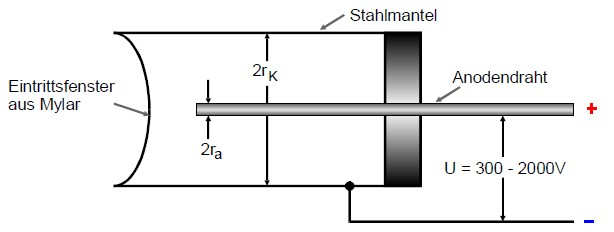
\includegraphics[height=5cm]{content/pics/gmz.jpg}
    \caption{Aufbau des Geiger-Müller-Zählrohrs \cite{v703}.}
    \label{fig:gmz}
\end{figure}

Sobald ein geladenes Teilchen, also auch $\alpha$- oder $\beta$-Teilchen, in das Zählrohr eindringt, wird dies
aufgrund von Ionisationsprozessen verlangsamt und schlussendlich absorbiert.
Die Anzahl von entstehenden Elektronen und positiven Ionen ist also auch proportional zur Energie der Strahlung,
da bei höherer kinetischer Energie mehr Ionisationsvorgänge stattfinden können, bevor diese aufgebraucht ist.
Die frei gewordenen Elektronen werden nun aufgrund der angelegten Spannung zur Anode beschleunigt.
Die dabei Ablaufenden Prozesse hängen stark von der Zählrohrspannung ab, in \autoref{fig:funktion} ist dieser
Zusammenhang graphisch dargestellt.

\begin{figure}[H]
    \centering
    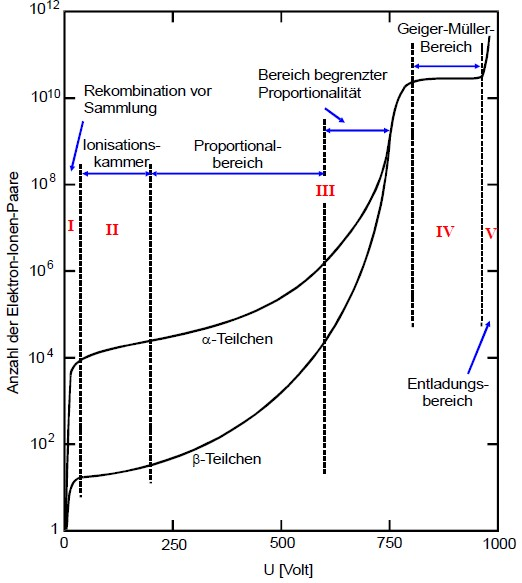
\includegraphics[height=9cm]{content/pics/funktion.jpg}
    \caption{Anzahl der erzeugten Elektron-Ionenpaare abhängig von der Zählrohrspannung $U$,
    für $\alpha$- und $\beta$-Teilchen \cite{v703}.}
    \label{fig:funktion}
\end{figure}

\begin{itemize}
\item Bei kleinen Zählrohrspannungen geht ein Großteil der Elektronen durch \textbf{Rekombination} verloren, somit
werden kaum Impulse gemessen.
\item Beim Erhöhen der Spannung fällt die Wahrscheinlichkeit einer Rekombination rasch ab,
sodass dann nahezu alle Elektronen die Anode erreichen. Der zwischen Kathode und Anode fließende
Ionisationsstrom ist proportional zur Energie bzw. zur Intensität der einfallenden Strahlung, unter diesen Umständen
wird das Geiger-Müller-Zählroh auch als \textbf{Ionisationskammer} bezeichnet.
\item Weiteres erhöhen von $U$ führt dazu, dass die Elektronen nach der primären Ionisation genug Energie gewinnen,
um selbst weitere Ionisationen auszulösen, dies wird auch als Stoßionisation bezeichnet. Dies führt schnell zu
lawinenartigen Kettenreaktionen, bei denen jedes Elektron weitere Elektronen auslöst. Insgesamt kommen dann
an der Anode so viele Elektronen an, dass ein Ladungsimpuls gemessen werden kann. Dieser Impuls ist proportional
zur Energie der einfallenden Strahlung und kann somit als Maß für diese verwendet werden. Aufgrund dieses Zusammenhangs
wird der Bereich auch als \textbf{Proportionalzählrohr} bezeichnet.
\item Eine Zählrohrspannung über dem Proportionalitätsbereich führt dazu, dass der Ladungsimpuls zunehmend unabhängig von der
Strahlungsenergie wird. Sobald ein konstantes Maximum erreicht ist, wird vom \textbf{Geiger-Müller-Bereich} gesprochen.
Hier werden nach jeder Primärionisation nahezu alle Gasatome im Zählrohr ebenfalls ionisiert, einerseits durch die bereits erwähnten
Elektronenlawinen und andererseits durch entstehende UV-Photonen. Diese Photonen sind eletrisch neutral und können sich somit durch das
gesamte Zählrohr bewegen und dort Ionisationen auslösen.
Eine Energiemessung der Strahlung ist hier nicht mehr möglich, es kann nur noch deren Intensität über die
Anzahl der Ladungsimpulse bestimmt werden.
\end{itemize}
Der von der Anode abfließende Strom ist proportional zur freigesetzten Ladungsmenge ($I = \dot{Q}$).
Sein Mittelwert kann mithilfe der in der Zeit $\symup{\Delta}t$ registrierten Teilchenzahl $Z$ und der pro Zeiteinheit
transportierten Ladungsmenge $\symup{\Delta}Q$ über 
\begin{equation}
  \label{eq:strom}
  \overline{I} = \frac{\symup{\Delta}Q}{\symup{\Delta}t}Z
\end{equation} 
berechnet werden.

\subsection{Totzeit und Nachentladung}
\label{sec:Totzeit}
Das Geiger-Müller-Zählrohr ist nicht in der Lage, eine unbegrenzte Menge an Signalen pro Zeiteinheit zu messen.
Während der sogenannten \textbf{Totzeit} direkt nach einer Ionisation schirmen die positiven Ionen das elektrische Feld der Anode ab
und verhinden somit die Messung eines weiteren Ladungsimpulses.
Erst wenn genügend der positiven Ionen zum Zählrohrmantel abgewandert sind und dort neutralisiert werden, kann ein neuer Impuls gemessen werden.
Eine Möglichkeit zur experiementellen Bestimmung der Totzeit $T$ besteht in der sogenannten \textit{Zwei-Quellen-Methode}.
Sind die einzeln Zählraten $N_1$ und $N_2$ von zwei unterschiedlichen Quellen sowie deren gemeinsame
Zählrate $N_{1,2}$ bekannt, so kann sie gemäß
\begin{equation}
    \label{eq:2 Quellen}
    T \approx \frac{N_1 + N_2 - N_{1,2}}{2N_1 N_2}
\end{equation}
angeschätzt werden.
Bevor sämtliche Ionen verschwunden sind, gibt es noch die sogenannte Erholungszeit, in der die gemessenen Impulse
geringere Beträge haben.

Ein weiterer Effekt ist die \textbf{Nachentladung}, die die gemessenen Zählraten verfälschen kann.
Durch auf den Zählrohrmantel treffende Ionen können sogenannte Sekundärelektronen freigesetzt werden, die
nach der Totzeit direkt wieder eine Ionisation im Zählrohr auslösen und somit die Messung von neuer Strahlung vortäuschen.
Um dies zu vermeiden, wird der bereits erwähnte Alkoholdampf eingesetzt. Die langkettigen Moleküle nehmen
die überschüssige Energie auf und verhindern die Emmision von Elektronen.

\subsection{Charakteristik des Zählrohres}
Die Charakteristik eines Geiger-Müller-Zählrohrs erhält durch Auftragen der registrierten Teilchenzahl $N$
gegen die Zählrohrspannung $U$, die Strahlungsintensität sei dabei konstant. Ein typischer Verlauf ist
in \autoref{fig:gmz charakteristik} dargestellt.

\begin{figure}[H]
    \centering
    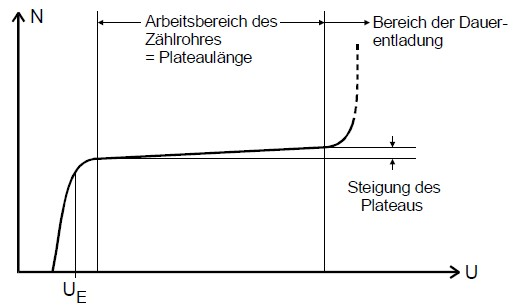
\includegraphics[height=5cm]{content/pics/charakteristik.jpg}
    \caption{Zählrohrcharakteristik bei konstanter Strahlungsintensität \cite{v703}.}
    \label{fig:gmz charakteristik}
\end{figure}

Ab der Spannung $U_\text{E}$ setzt der Auslösebereich ein, darauf folgt ein \textbf{Plateau}.
Optimalerweise sollte das Plateau keine Steigung aufweisen, doch in der Praxis ist aufgrund
einiger wenigen Nachentladungen trotzdem ein kleiner Anstieg zu beobachten.
Diese Steigung ist ein Maß für die Qualität des Zählrohrs, da ein längeres und flacheres
Plateau bessere Messwerte garantiert.
Am Ende des Plateaus beginnt die Zahl der Nachentladungen stark zu steigen, bis es schlussendlich
zur selbstständigen Gasentladung kommt.
Hier wird durch ein einziges ionisierendes Teilchen eine Dauerentladung gezündet, sodass das
Zählrohr unbrauchbar wird.